\chapter{Tranzystor grafenowy}

Jak to działo się wiele razy w historii pojedyncze odkrycie, rzeczy z pozoru błahej daje początek
nowej idei, która staje się nowym kołem zamachowym dalszego rozwoju. Być może znajdujemy się 
w przededniu takiego odkrycia, porównywalnego do wynalezienia tranzystora. Mowa tutaj o grafenie, 
który jest bardo poważnym kandydatem na materiał w erze elektroniki post-krzemowej. 
Jako dowód tego stwierdzenia wystarczy wspomnieć, że grafen znajduje się na liście 
,,Międzynarodowej mapie technologii półprzewodnikowej" \footnote{The International Technology Roadmap for Semiconductors http://www.itrs.net/
Links/2009ITRS/Home2009.htm (Semiconductor Industry Association, 2009).}

Dzięki wzmożonej pracy wielu zespołów naukowych badających grafen. Już dzisiaj można mówić o realnej 
możliwości zastosowania tego materiału w procesie produkcji urządzeń elektronicznych. Mimo tak szybkiego 
rozwoju tej tematyki nie można w sposób jednoznaczny rozstrzygnąć panującej dyskusji, czy jest to na 
pewno wykonalne. 

W niniejszym rozdziale zostanie przedstawiona idea działania tranzystora FET. Prawdopodobnie najlepszej 
koncepcji urządzenia elektronicznego w dzisiejszym świecie. Następnie zostanie przedstawiona koncepcja 
zastosowania grafenu przy produkcji tego typu urządzenia. Wraz z omówieniem podstaw fizycznych jego działania,
modelami teoretycznymi, zostaną również przedstawione najważniejsze parametry z punktu widzenia inżynierii
stosowania takich urządzeń. Modele teoretyczne posłużą w następnym rozdziale do ich konfrontacji z danymi
eksperymentalnymi. Co zostanie opisane w następnym rozdziale. Na koniec zostanie przedstawiony proces 
wytwarzania takiego tranzystora.



	\section{Tranzystor FET}
Nazwa tego typu urządzenia pochodzi od angielskiego \textit{Field Effect Transistor}. Ze względu na największe
podobieństwo konstrukcji tranzystorów grafenowych do tranzystorów polowych typu MOSFET (\textit{ Metal-Oxide-Semi
conductur FET}), stanie się on podstawowym punktem odniesienia.
Budowa takiego urządzenie została przedstawiona na rysunku \ref{fig:MOSFET}. 


	\begin{figure}[ht]
	\centering
	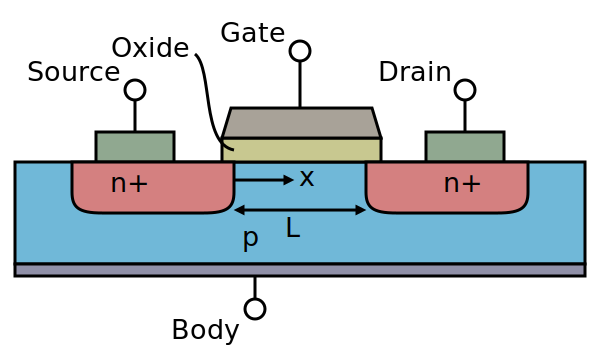
\includegraphics[width=0.50\textwidth]{./Rozdzial_3/obrazki/Lateral_mosfet}
	\caption{Przekrój ukazujący wewnętrzna budowę tranzystora typu MOSFET}
	\label{fig:MOSFET}
	\end{figure}

Jak widzimy na podłożu typu p zostały wytworzone obszary typu n, stanowiące źródło i dren. Zazwyczaj obszary te 
powstają na drodze implantacji jonów lub dyfuzji atomów domieszek do podłoża. Pomiędzy tymi obszarami w efekcie 
zjawiska polowego powstaje kanał. Kanał tworzy  się, gdy pomiędzy bramkę a podłoże zostanie przyłożone napięcie. 
Dla tranzystora typu n-kanałowego, napięcie musi być dodatnie. Po przyłożeniu dodatniego napięcia, elektrony 
z podłoża zaczynają gromadzić się pod bramką. W ten sposób jako nośniki mniejszościowe sprawiają, że obszar ten
staje się obszarem wyróżnionym pod względem zwiększenia jego przewodności. Dzięki temu przy przyłożonym napięciu 
pomiędzy drenem a źródłem zaczyna płynąć prąd. 

Taki tranzystor może znajdować się w 3 obszarach pracy. Wyłączony, brak wytworzonego kanału, duża oporność pomiędzy
drenem i źródłem. Obszar liniowej pracy kiedy to prąd drenu zależy w przybliżeniu liniowo od napięcia dren-źródło. 
Wreszcie obszar nasycenia, gdzie prąd źródło-dren słabo zależy od zmian napięcia pomiędzy nimi. Wszystkie te sytuacje
przedstawia rysunek \ref{fig:MOSFET_char}.


	\begin{figure}[ht]
	\centering
	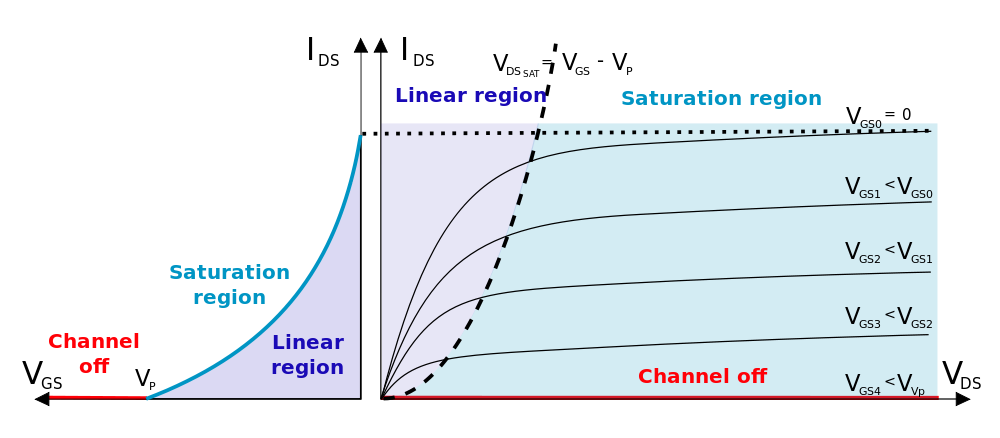
\includegraphics[width=0.90\textwidth]{./Rozdzial_3/obrazki/Charakterystyki_FET}
	\caption{Zależność prądu płynącego przez tranzystor}
	\label{fig:MOSFET_char}
	\end{figure}

Matematycznie można to opisać równaniem:

\begin{equation}
    \mathrm{ I_{DS}(V_G, V_{DS}) = \mu C_{ox} \frac{W}{L}[(V_G - V_T)V_{DS} - \frac{V_{DS}^2}{2}]}
	\label{equ:prad_drenu}
\end{equation}

Wyróżniamy dwa podstawowe typy charakterystyk elektrycznych tranzystorów FET. Pierwszym jest charakterystyka przejściowa,
którą otrzymuje się gdy prąd drenu otrzymuje się jako funkcję napięcia bramkowego, przy stałym napięciu źródło-dren. 
Drugim typem jest tak zwana charakterystyka wyjściowa będąca funkcją prądu drenu do napięcia dren-źródło, przy stałym 
napięciu bramkowym.

Mierząc te charakterystyki i porównując je ze wzorem \ref{equ:prad_drenu}, można wyznaczyć ruchliwość badanego tranzystora, $\mu$. 
Znając inne parametry występujące we wzorze, gdzie: L-długość kanału, W-szerokość kanału, 
$\mathrm {C_{ox}}$-powierzchniowa gęstość
 pojemności pomiędzy kanałem a bramką, $\mathrm{ V_G}$-napięcie bramkowe,
 $\mathrm{ V_{DS}}$-napięcie dren-źródło, $\mathrm{ V_T}$-tak zwane napięcie progowe.
Pomiary tych charakterystyk stały się podstawą do wyciągnięcia wniosków o właściwościach transportowych grafenu, użytego
w roli kanału.

Dzisiaj w świecie inżynierii elektronicznej istnieją dwie podstawowe grupy określające zastosowanie danego tranzystora. 
Zastosowania w układach logicznych lub w układach radiowych. W zasadzie można powiedzieć, że albo do zastosowań cyfrowych
albo do zastosowań analogowych. 

Relatywnie większą łatwość wprowadzania nowych technologicznie materiałów obserwuje się w segmencie analogowym. Wynika, to
głównie z tego względu, że wydajność urządzeń cyfrowych najbardziej zależy od najgorszych egzemplarzy tranzystorów 
zintegrowanych w układzie logicznym. Podczas, gdy w przypadku pojedynczo produkowanych tranzystorów do zastosowań analogowych,
te z nich, które za bardzo odbiegają parametrami od norm mogą zostać niedopuszczone do sprzedaży. Co odbywa się bez wpływu
dla reszty sprzedawanych egzemplarzy tranzystorów. To samo tyczy się zintegrowanych układów scalonych. Jako znacznie
prostsze są mniej narażone na ewentualne odchyłki parametrów pojedynczego tranzystora.

Jednak pomimo różnic, obie te gałęzie dążą do wspólnych celów. Zmniejszenia kosztów produkcji pojedynczego tranzystora.
Polepszenia jego właściwości. Głównie dla tranzystorów przeznaczonych do zastosowań cyfrowych działaniem mającym na celu
 zaspokojenie obu tych wymagań przez wiele lat było sukcesywne zmniejszanie pojedynczego tranzystora. Dzięki temu stawały
 się one szybsze. Zajmując mniej miejsca na podłożu oszczędzały drogi krzem.

Dzięki tym zabiegom złożoność układów cyfrowych mogła się podwajać co 18 miesięcy. Ta zależność jest nazywana ,,prawem
Moora". Jednocześnie takie układy stawały się tańsze.

Ze zmniejszaniem się pojedynczego tranzystora rosły wymagania co do procesu technologicznego, w którym je produkowano.
Dzisiejsze fabryki układów scalonych stały się niesłychanie kosztownymi przedsięwzięciami (kosztującymi miliardy dolarów).
Właśnie te linie produkcyjne są jednym z powodów całkowitego opanowania przez krzem technologii produkcji układów
 cyfrowych, ponieważ budowa nowej fabryki pochłonie więcej pieniędzy niż modernizacja obecnej. Należy pamiętać, że postępem
rządzi ekonomia.

To rozwiązanie zaczęło zawodzić, kiedy zaczęto dochodzić rozmiarami tranzystora do granic możliwości. Wtedy stało się jasne,
że niezbędne będzie opracowanie całkowicie nowej technologii wytwarzania lepszych tranzystorów.

Wspomniana technologia układów cyfrowych opiera się na komplementarnych tranzystorach CMOS (\textit{Complementary Metal-
Oxide-Semiconductur}). Podstawowym budulcem bramek logicznych jest para tranzystorów MOS z kanałami n i p. Oba mogą 
znajdować w dwóch stanach: włączenia i wyłączenia. Najwięcej energii pobierane jest, gdy chcemy zmienić ten stan. 
Idea polega na takim projektowaniu układów logicznych by poszczególne bramki logiczne składały się z kombinacji
tranzystorów n i p kanałowych, która zapewnia brak przepływu dużych prądów w stanie ustalonym. Często najbardziej znaczącym
prądem w stanie ustalonym jest suma prądów upływności bramek. Są one niezbędne do poprawnej polaryzacji bramki.
Z tego powodu bardzo pożądaną właściwością tych tranzystorów jest duży stosunek prądu włączenia do prądu wyłączenia, z 
warunkiem minimalizacji prądu wyłączenia. Typowymi wartościami są tutaj stosunki wł/wył wynoszące 10$^4$--10$^7$
\footnote{gr. tranz. ref 2}.  W typowych konstrukcjach poszczególnych FET-ów wymaga to posiadania wystarczająco szerokiej
przerwy energetycznej najlepiej więcej niż 0,4 eV. Drugą ważną właściwością jest posiadanie dokładnie takiego samego
napięcia przełączania. Dopiero te dwa warunki są w stanie zapewnić dobrego kandydata na następce dla dzisiaj stosowanych
materiałów.


Sytuacja w dziedzinie zastosowań analogowych, ze szczególnym wskazaniem zastosowań radiowych, wygląda z goła inaczej. 
Tutaj sama miniaturyzacja tranzystora nie jest najważniejsza, bo ważniejsze są jego właściwości, a same zintegrowane układy
analogowe są znacznie bardziej proste niż cyfrowe. Dodatkowo badania nad wieloma technologiami były i są wspierane przez
 agencje wojskowe. Dzięki temu produkty wysokiej jakości, ale będące drogie znajdują swoje zastosowania. Dzięki temu ten
 segment rynku jest znacznie bardziej otwarty na nowe technologie. Jako przykłady można wspomnieć tutaj np o tranzystorach
HEMT, opartych na materiałach III-IV; urządzeniach opartych na technologii arsenku galu GaAs, lub fosforku indu InP.


W zastosowaniach analogowych nie wymaga się od tranzystora posiadania stanu całkowitego wyłączenia. Zazwyczaj i tak 
w większości zastosowań tranzystory te pracują w jakimś punkcie pracy, który wymusza stały przepływ prądu. Tutaj dużo 
ważniejszym parametrem jest z kolei liniowość i wysoka częstotliwość odcięcia. W przypadku grafenu co zostanie pokazane
poniżej warunek liniowości jest bardzo dobrze spełniony. Tak samo jak spełniony jest ten o wysokiej częstotliwości odcięcia.
Donosi się o tranzystorach grafenowych o specjalnej budowie, gdzie rolę bramki pełni nanoprzewód, dla których
częstotliwość odcięcia zawierała się w przedziale 100--300 GHz \footnote{High-speed graphene transistors with a self-aligned nanowire gate}.



Podsumowując, z powodów tutaj przedstawionych wynika, że technologia grafenu ma większą szansę zaistnieć 
w wysokoczęstotliwościowych zastosowaniach analogowych. Dodatkowe argumenty potwierdzające tą tezę znajdują się 
w kolejnej części, mówiącej o czysto fizycznych aspektach stosowania grafenu do produkcji urządzeń elektronicznych.

	\section{Tranzystor FET z kanałem grafenowym}
		\subsection{Podstawy fizyczne działania}	
	W szerokich paskach grafenowych może istnieć wile pojedynczych kanałów przewodnictwa. Transport przez te kanały
	jest proporcjonalnie zmniejszany względem długości całego paska. Szerokość natomiast ma wpływ na wzrost liczby
	dostępnych kanałów. Zakładając, że mówimy tutaj o sytuacji, w której znajdujemy się w pobliżu punktów Diraca.
	Można napisać, że:

	\begin{equation}
    		\mathrm{ G \sim \frac{e^2}{h}\frac{W}{L} }
		\label{equ:G}
	\end{equation}
	Gdzie W-szerokość paska grafenowego, L-jego długość. Wzór \ref{equ:G}, pochodzi z \footnote{http://arxiv.org/abs/cond-mat/0603315}.
	Ta zależność prowadzi do wniosku, że przewodność skaluje się tutaj tak jak w przypadku funkcji przewodnictwa w 
	metalach dyfuzyjnych. 


		\begin{figure}[ht]
	\centering
	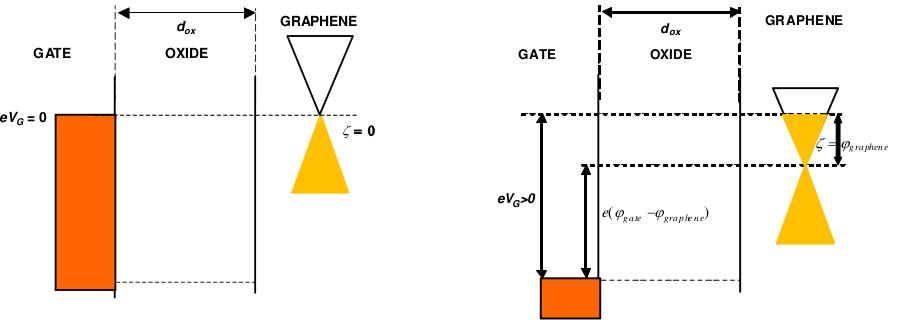
\includegraphics[width=0.90\textwidth]{./Rozdzial_3/obrazki/zasadadzialania.jpg}
	\caption{Zasada działania tranzystora grafenowego}
	\label{fig:MOSFET_dzialanie}
	\end{figure}

DOKŁADNY OPIS TEGO OBRAZKA TERAZ!!!!!!!
	
	Zależność koncentracji od napięcia bramkowego jest liniowa, a koncentracja wiąże się również liniowo z 
	przewodnictwem\footnote{http://jpsj.ipap.jp/link?JPSJ/71/1318/}. Co zostało zaprezentowane w poprzednim rozdziale.
	 Z tego wynika, że zależność przewodności jest liniową funkcją napięcia bramkowego co zostało pokazane empirycznie
	np. przez \footnote{http://www.ncbi.nlm.nih.gov/pmc/articles/PMC1180777/}.
	Jedynym miejscem, gdzie nie jest to prawdą jest okolica występowania minima przewodnictwa. Jest to związane, ze 
	zmianą typów nośników. 

	
	



		\subsection{Najważniejsze właściwości}
			\paragraph{Ruchliwość}


	Jest to najczęściej podawana zaleta grafenu. Zwłaszcza zdolność do jej zachowania nawet w temperaturach 
	pokojowych, co zostało omówione w poprzednim rozdziale, wraz z podaniem jej wartości dla poszczególnych 
	przypadków grafenu na różnych podłożach.
	Wysokie wartości osiąganych ruchliwości w tym materiale robią duże nadzieje na znalezienie dla tego materiału
	odpowiedniego zastosowania. 
	
	Problemem jest tutaj to, że tak duże wartości są osiągane dla dużych próbek grafenu, które z kolei nie posiadają 
	przerwy energetycznej. Jest to znaczna wada, co zostało wykazane w poprzednim podpunkcie. 
			\paragraph{Przerwa energetyczna}


	Jak zostało wspomniane przerwa energetyczna jest bardo pożądaną własnością. Powody zostały przedstawione na początku
	tego rozdziału. Istnieją metody takiej inżynierii grafenu, zdolne wytworzyć przerwę energetyczną w grafenie. 
	Jednak skutkuje to bardzo znacznym zmniejszeniem ruchliwości, czyli głównej zalety tego materiału.
	Mówiąc bardziej ilościowo, dla metody stosowania tak zwanych nanowstążek grafenowych ruchliwości wynoszą około 
	200 $\mathrm{\frac{cm^2}{V s}}$, co jest wielkością o trzy rzędy większości mniejszą niż w grafenie pochodzącym
	z eksfoliacji, o dużo większej powierzchni. \footnote{tutaj odnośniki z 1 rozdziału}

Dlatego podsumowując najlepiej było by opracować taką technologię, która wymaga wysokiej ruchliwości i nie wymaga posiadania
przerwy energetycznej. Zamiast przystosowywać ten materiału do znanych nam obecnie technologii. Dlatego w dalszym ciągu
ewentualne zastosowania w przemyśle pozostają kwestią otwartą.



		\subsection{Omówienie charakterystyk elektrycznych}
			\paragraph{Ogólny wygląd}

	\begin{figure}[ht]
	\centering
	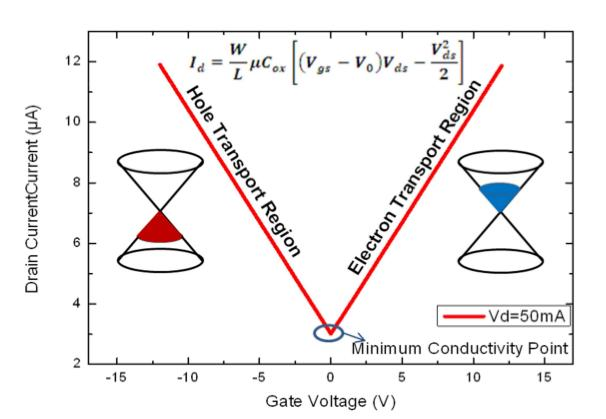
\includegraphics[width=0.90\textwidth]{./Rozdzial_3/obrazki/charakterystykaPrzej}
	\caption{Wygląd typowej charakterystyki przejściowej tranzystora GFET}
	\label{fig:GFET_trans} 
	\end{figure}

Pierwszą i mającą w zasadzie największe znaczenie dla wyznaczania najważniejszych parametrów charakteryzujących tranzystory 
jest charakterystyka przejściowa. Charakterystyka przejściowa zbierana jest, gdy mierzony jest prąd płynący przez kanał, 
przy stałym napięciu dren-źródło w funkcji napięcia bramkowego. Często prąd zamieniany jest na wielkość zapewniającą
bardziej obiektywny wgląd w faktyczne zmiany właściwości materiału jaką jest przewodność, ewentualnie rezystywność. 
Taka typowa charakterystyka została przedstawiona na obrazku \ref{fig:GFET_trans}. Jak widać, charakterystyka jest liniowo 
zależna od napięcia bramkowego, oprócz obszaru w okolicy minimum przewodnictwa. 


	\begin{figure}[ht]
	\centering
	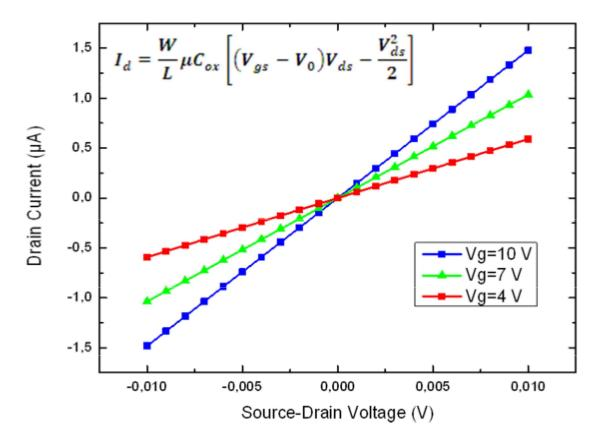
\includegraphics[width=0.90\textwidth]{./Rozdzial_3/obrazki/charakterystykaWyj.jpg}
	\caption{Wygląd typowej charakterystyki wyjściowej tranzystora GFET}
	\label{fig:GFET_out} 
	\end{figure}

Drugim typem charakterystyki jest charakterystyka wyjściowa. Pomiarów tej charakterystyki dokonuje się poprzez 
Ustawienie stałego napięcia bramkowego i wyznaczeniu prądu dren-źródło w funkcji napięcia dren-źródło. Typowy wygląd 
charakterystyki dla grafenu został przedstawiony na rysunku \ref{fig:GFET_out}. Tutaj również często zamienia się prąd na
przewodność lub rezystywność. Ten rodzaj charakterystyki zazwyczaj ma mniejsze znacznie dla charakteryzacji.

\subsection{Proponowane modele transportu}
W niniejszej pracy zaprezentowano kilka najczęściej proponowanych podjeść do wyznaczania parametrów transportowych urządzeń
grafenowych. Głównym parametrem wyznaczanym dla tych urządzeń jest ruchliwość. Istnieją co najmniej trzy metody jej 
wyznaczania. 
\paragraph{Model Drudego}

Pierwszym z modeli transportu jest model Drudego. Model Drudego zazwyczaj znajduje zastosowanie w opisie metali. Grafen 
jest półmetalem dlatego istnieją przesłanki do jego stosowania. Model ten opiera się na kinetycznej teorii gazów, gdzie
zamiast gazu mamy do czynienia z tak zwanym gazem elektronowym. Elektrony tak jak molekuły gazu poruszają się chaotycznie
zderzając się z jonami sieci krystalicznej. Po przyłożeniu pola elektrycznego powstaje kolektywny ruch w kierunku działania 
pola, który jest nałożony na te chaotyczne drgania termiczne. 
W ogólności można zapisać:

\begin{equation}
    \mathrm{ \vec J =q n_{ind} \mu_{Drude} \vec E }
\end{equation}

Z tego równania na gęstość prądu można po prostych przekształceniach otrzymać równanie używane do określenia ruchliwości 
dla próbek grafenowych:

\begin{equation}
   \mathrm{ \sigma = C_{ox}} V_G\mathrm{ \mu_{Drude}}
	\label{equ:przewodnoscDrudego}
\end{equation}

Gdzie C$_{ox}$-gęstość powierzchniowa pojemności, opisana wzorem:
\begin{equation}
   \mathrm{C_{ox}= \frac {\epsilon_o \epsilon_r}{d_{ox}}}
\end{equation}

Dzięki temu funkcja przewodności $\sigma$, zależy tylko od jednego parametru w sposób liniowy. To znaczy od napięcia
bramkowego $V_G$. Mając takie opis matematyczny i dysponując zmierzonymi charakterystykami przejściowymi, wyznaczenia
ruchliwości dokonuje się dopasowywyjąc zmierzoną przewodność do tej oczekiwanej. Parametrem dopasowywanym jest oczywiście
ruchliwość, ponieważ inne zmienne występujące w równaniu \ref{equ:przewodnoscDrudego}, są albo znane.

Dla tego modelu donosi się o wysokich ruchliwościach przy wysokiej koncentracji nośników. \footnote{1,17 model tr. gr.}

\paragraph{Model stałej ruchliwości}
Model zakładający stałą ruchliwość nośników w grafenie, niezależnej od koncentracji, zaproponowany został przez 
\footnote{S. Adam, E. H. Hwang, and S. Das Sarma, Physica E 40, 1022 (2008).}. 
Dzięki takim założeniom można zapisać wzór na opór elektryczny próbki jako :

\begin{equation}
    \mathrm{ R_{całkowite} = 2R_{kontakt}+ \frac{L}{W}\frac{1}{\mu \sqrt{e^2 n_o + C_{ox}^2(V_G-V_{Dirac}^2)}}}
	\label{equ:stalaRuch}
\end{equation}

W przypadku równania \ref{equ:stalaRuch} również dopasowywuje się to równanie do danych eksperymentalnych. Parametrami
dopasowania są w tym przypadku: R$_{kontatkt}$-będące opornością kontaktów, stałą ruchliwość $\mu$  i koncentrację nośników
n$_o$.

\paragraph{Model ruchliwości Halla}
Ta metoda wyznaczania ruchliwości jest również często stosowana, choć wymaga ona dodatkowego sprzętu laboratoryjnego. 
Przedstawiając w sposób najprostszy polega ona na wyznaczaniu zależności oporu przy stałych napięciach bramkowych
w obecności zmiennych pól magnetycznych. 

Ta metoda nie znalazła zastosowania w niniejszej pracy. Dlatego nie zostanie ona opisana dokładniej.

\paragraph{Metoda techniczna (to jest chyba do zmiany!)}
Istnieje jeszcze metoda wykorzystująca ogólny model tranzystora FET. Opisany równaniem \ref{equ:prad_drenu}, gdzie po 
prostych przekształceniach i założeniu, że znajdujemy się w liniowym obszarze charakterystyki przejsciowej, można napisać:

\begin{equation}
    \mathrm{ \mu_{FE} = \frac{L}{W}\frac{g_m}{C_{ox}V_{DS}}}
\end{equation}
\begin{equation}
    \mathrm{ g_m = \frac{d I_D}{d V_G} |_{ V_{DS}=const}}
\end{equation}

Ogromną zaletą tej metody jest jej uniwersalność i możliwość porównywania tranzystorów wykonanych nawet w zupełnie innej
technologii i przy użyciu innych materiałów. 

Nie jest ona niestety pozbawiona wad. Duży wpływ na wartość otrzymanej ruchliwości ma wybór części charakterystyki. 
Dlatego istnieje tutaj sporo miejsca do nadużyć, lub popełniania błędów. Jednak w przypadku urządzeń grafenowych, nie ma
to aż takiego znaczenia, ponieważ te charakterystyki są liniowe w szerokim zakresie. Dlatego również ta metoda jest dobra
do oszacowania ruchliwości.

	\section{Najnowsze technologie tranzystorów grafenowych}

	\section{Proces produkcji tranzystorów z kanałem grafenowym}
		\subsection{Struktury tranzystorów}
		\subsection{Metoda produkcji tranzystorów}
			\paragraph{Opis metodologii}
			\paragraph{Zdjęcia optyczne}
